% ============================================================================
% CS4052 - Computación Paralela y Distribuida (2026-II) - UTEC
% Proyecto 5: KNN sobre load_digits mediante MPI (mpi4py) -- INFORME FINAL
% Compilar: pdflatex -> biber -> pdflatex -> pdflatex
% Estructura de carpetas esperada:
%   latex/informe_final.tex, latex/algoritmos_pram.tex, latex/refs.bib
%   figures/*.pdf     (generadas por src/generate_plots.py)
% ============================================================================
\documentclass[11pt,a4paper]{article}

\usepackage[T1]{fontenc}
\usepackage[utf8]{inputenc}
\usepackage[spanish,es-tabla,es-noshorthands]{babel}
\usepackage[a4paper,margin=2.5cm]{geometry}
\usepackage{amsmath,amssymb}
\usepackage{graphicx}
\usepackage{booktabs}
\usepackage{multirow}
\usepackage{array}
\usepackage{tabularx}
\usepackage{xcolor}
\usepackage{caption}
\usepackage{subcaption}
\usepackage{float}
\usepackage{listings}
\usepackage[ruled,linesnumbered,noend]{algorithm2e}
\usepackage[backend=biber,style=numeric,sorting=none]{biblatex}
\usepackage{csquotes}
\usepackage[hidelinks]{hyperref}

\addbibresource{refs.bib}
\setlength{\emergencystretch}{3em}   % evita desbordes con identificadores en \texttt
\Urlmuskip=0mu plus 1mu
\graphicspath{{../figures/}}

% ---------------------------------------------------------------- algorithm2e
\SetKwFor{ForAllPar}{forall}{pardo}{end}
\SetKwInput{KwLocal}{Datos locales}
\SetKwInput{KwShared}{Memoria global}
\SetKwComment{tcp}{$\triangleright$\ }{}
\SetKwFunction{Bcast}{Bcast}\SetKwFunction{Scatterv}{Scatterv}
\SetKwFunction{Gather}{Gather}\SetKwFunction{Gatherv}{Gatherv}
\SetKwFunction{Predict}{knn\_predict}\SetKwFunction{Dist}{Distancia}

% ---------------------------------------------------------------- listings
\definecolor{codebg}{RGB}{248,248,246}
\definecolor{codekw}{RGB}{0,82,147}
\definecolor{codecm}{RGB}{110,110,110}
\definecolor{codestr}{RGB}{163,21,21}
\lstset{
  language=Python, basicstyle=\ttfamily\footnotesize, backgroundcolor=\color{codebg},
  keywordstyle=\color{codekw}\bfseries, commentstyle=\color{codecm}\itshape,
  stringstyle=\color{codestr}, numbers=left, numberstyle=\tiny\color{codecm},
  frame=single, rulecolor=\color{codecm!40}, breaklines=true, columns=fullflexible,
  showstringspaces=false, xleftmargin=1.5em, framexleftmargin=1.5em,
  literate={á}{{\'a}}1 {é}{{\'e}}1 {í}{{\'i}}1 {ó}{{\'o}}1 {ú}{{\'u}}1 {ñ}{{\~n}}1
           {Á}{{\'A}}1 {É}{{\'E}}1 {Í}{{\'I}}1 {Ó}{{\'O}}1 {Ú}{{\'U}}1
}

\newcommand{\ntr}{n_{\text{train}}}
\newcommand{\mte}{m_{\text{test}}}
\newcommand{\Xtr}{X_{\text{tr}}}
\newcommand{\Xte}{X_{\text{te}}}
\newcommand{\ytr}{y_{\text{tr}}}
\newcommand{\yte}{y_{\text{te}}}
\newcommand{\Tcomp}{T_{\text{comp}}}
\newcommand{\Tcomm}{T_{\text{comm}}}
\newcommand{\Ttot}{T_{\text{total}}}

\begin{document}

% ============================================================================
% PORTADA
% ============================================================================
\hypersetup{pageanchor=false}
\begin{titlepage}
\centering
{\large Universidad de Ingeniería y Tecnología (UTEC)\par}
{\large Facultad de Ciencia de la Computación\par}
\vspace{0.4cm}
{CS4052 -- Computación Paralela y Distribuida -- 2026-II\par}
\vspace{2.5cm}
{\Large Informe final de proyecto\par}
\vspace{0.6cm}
{\LARGE\bfseries Proyecto 5: paralelización del clasificador KNN\\[0.2cm]
sobre \texttt{load\_digits} mediante MPI (\texttt{mpi4py})\par}
\vspace{2.5cm}
{\large\bfseries Integrantes:\par}
\vspace{0.3cm}
\begin{tabular}{lr}
Juan David Velo Poma & (100\,\%)\\
Farid Jack Aquino Castro & (100\,\%)\\
Josue Nehemias Velo Poma & (100\,\%)\\
\end{tabular}
\vfill
{\large\bfseries Profesor:\par}
{José Fiestas, PhD\par}
\vspace{0.8cm}
{\large\bfseries Entrega:\par}
{Noviembre de 2026\par}
\end{titlepage}
\hypersetup{pageanchor=true}

\tableofcontents
\newpage

% ============================================================================
\section{Introducción}
% ============================================================================

\subsection{El problema y el algoritmo elegido}
El algoritmo de $k$ vecinos más cercanos (KNN), propuesto por Fix y Hodges~\cite{fix1951} y
caracterizado formalmente por Cover y Hart~\cite{cover1967}, es un clasificador supervisado no
paramétrico: no construye un modelo durante el entrenamiento y difiere todo el cómputo al momento
de la consulta. Para clasificar $q\in\mathbb{R}^d$ se calcula su distancia a los $\ntr$ puntos
etiquetados, se eligen los $k$ más cercanos y se asigna la etiqueta mayoritaria.

Este perfil ---entrenamiento gratuito, inferencia costosa--- lo hace idóneo para el cómputo
paralelo: el trabajo se concentra en una región bien identificada (las $\mte\cdot\ntr$
distancias) y cada consulta es independiente de las demás. En el modelo DAG del curso, el problema
es un algoritmo secuencial--paralelo: distribución de datos, una fase masivamente paralela y
recolección de resultados~\cite{fiestasU1}.

\subsection{Código secuencial de partida}
El archivo \texttt{knn\_digits\_sec.py} del enunciado~\cite{fiestasProyecto} usa
\texttt{load\_digits}~\cite{pedregosa2011,alpaydin1998}: 1797 imágenes de $8\times 8$ píxeles con
valores en $[0,16]$ ($d=64$, $C=10$ clases). Con \texttt{test\_size=0.2} y
\texttt{random\_state=42} se obtiene $\ntr=1437$ y $\mte=360$, y se fija $k=3$. La función
\texttt{knn\_predict} recorre en un bucle de Python los $\ntr$ puntos calculando
\begin{equation}
  d(q,x)=\sqrt{\sum_{l=1}^{d}(q_l-x_l)^2},\label{eq:dist}
\end{equation}
ordena las distancias con \texttt{np.argsort} y vota con \texttt{Counter}. Su exactitud es
$0.9833$ y su tiempo, $T_s=1.40$\,s en la plataforma de la Sec.~\ref{sec:entorno}.

\subsection{Solución planteada}
Se descompone el dominio de consultas: $\Xte$ se reparte en bloques disjuntos entre los $s$
procesos MPI y $\Xtr$, que todo proceso necesita íntegro, se replica con una difusión
(\texttt{bcast}/\texttt{Bcast}). Las predicciones locales se recolectan con
\texttt{gather}/\texttt{Gatherv}. Además, cumpliendo lo anunciado en el informe parcial, se
implementa la descomposición alternativa del DAG del enunciado ---reparto de $\Xtr$, difusión de
$\Xte$ y fusión de candidatos--- y se comparan ambas experimentalmente.

El desarrollo se registra en tres versiones beta (Sec.~\ref{sec:codigo}). Como \texttt{load\_digits}
se resuelve en milisegundos y el arranque de MPI dominaría las mediciones, se generan conjuntos
sintéticos de hasta $N=245\,000$ muestras con la misma estadística por clase
(Sec.~\ref{sec:datos}).

% ============================================================================
\section{Método}
% ============================================================================

\subsection{Notación}
\begin{table}[H]
\centering
\caption{Notación empleada en todo el informe (idéntica al informe parcial).}
\label{tab:notacion}
\begin{tabular}{ll}
\toprule
Símbolo & Significado\\
\midrule
$\ntr$ (o $n$) & puntos de entrenamiento\\
$\mte$ (o $m$) & puntos de prueba (consultas)\\
$N=\ntr+\mte$ & tamaño total del conjunto ($\ntr=0.8N$)\\
$d$ & dimensión del espacio de características ($d=64$)\\
$k$ & número de vecinos ($k=3$)\\
$s$ & número de procesos MPI (el $p$ del enunciado)\\
$p$ & rango de un proceso, $p\in\{0,\dots,s-1\}$\\
$m_p$, $\mathrm{displ}_p$ & consultas asignadas al proceso $p$ y su desplazamiento\\
$\alpha$, $\beta$ & latencia por mensaje y tiempo por palabra\\
$W$, $T_\infty$ & trabajo y span (camino crítico)\\
$T_s$, $T_p(s)$ & tiempo secuencial y paralelo con $s$ procesos\\
$\Tcomp$, $\Tcomm$ & tiempos de cómputo y de comunicación\\
$S(s)$, $E(s)$ & speedup y eficiencia\\
$f_s$, $f_p$ & fracciones serial y paralela ($f_s+f_p=1$)\\
$k_1$, $k_2$ & constantes de normalización del modelo teórico\\
\bottomrule
\end{tabular}
\end{table}

\subsection{Metodología de Foster (PCAM) y modelo de ejecución}
El diseño sigue la metodología de Foster~\cite{foster1995,fiestasU1}:
\begin{enumerate}
  \item \textbf{Particionamiento.} La tarea primitiva es el cálculo de la distancia
        (Ec.~\ref{eq:dist}) entre una consulta y un punto de entrenamiento: $\mte\cdot\ntr$ tareas.
  \item \textbf{Comunicación.} Todas las tareas de una consulta leen $\Xtr$ completo
        (comunicación global $\Rightarrow$ \texttt{Bcast}); cada consulta se envía a un solo
        proceso (\texttt{Scatterv}); cada etiqueta predicha vuelve a la raíz (\texttt{Gatherv}).
  \item \textbf{Aglomeración.} Las $\ntr$ distancias de una consulta y las $m_p\approx\mte/s$
        consultas de un bloque se agrupan en un proceso, maximizando la granularidad
        $G=\Tcomp/\Tcomm$.
  \item \textbf{Mapeo.} Un proceso MPI por núcleo lógico del procesador multinúcleo, con
        reparto por bloques que admite $\mte \bmod s\neq 0$.
\end{enumerate}
En la taxonomía de Flynn~\cite{flynn1972} el sistema es MIMD con paradigma SPMD: los $s$
procesos ejecutan el mismo programa sobre datos distintos.

\subsection{Pseudocódigos: secuencial, PRAM y distribuido con \texttt{pardo}}
\label{sec:pseudo}
Los Algoritmos~\ref{alg:dist}--\ref{alg:knn-sec} describen el código secuencial. Atendiendo la
retroalimentación de la entrega parcial, \textbf{todos los bucles concurrentes se escriben con el
formalismo \texttt{forall}~\ldots~\texttt{pardo}}~\cite{jaja1992,fiestasU22}: en la PRAM
(Algoritmo~\ref{alg:knn-pram}) y en las dos versiones distribuidas
(Algoritmos~\ref{alg:knn-mpi} y~\ref{alg:knn-dag}).

\begin{algorithm}[H]
\caption{Distancia euclidiana}\label{alg:dist}
\KwIn{Dos arreglos $a,b\in\mathbb{R}^d$}
\KwOut{Distancia $\|a-b\|_2$}
$\delta\leftarrow 0$\;
\For{$i\leftarrow 0$ \KwTo $d-1$}{
  $\delta\leftarrow\delta+(a[i]-b[i])^2$\;
}
\Return{$\sqrt{\delta}$}\;
\end{algorithm}

\begin{algorithm}[H]
\caption{KNN predict}\label{alg:predict}
\KwIn{Punto de prueba $x_{\text{test}}\in\mathbb{R}^d$, $\Xtr\in\mathbb{R}^{\ntr\times d}$,
      $\ytr\in\{0,\dots,9\}^{\ntr}$, número de vecinos $k$}
\KwOut{Etiqueta predicha $\hat{y}$ (moda de los $k$ vecinos más cercanos)}
$D\leftarrow[\,]$\;
\ForEach{$x_{\text{punto}}\in\Xtr$}{
  añadir \Dist{$x_{\text{test}}, x_{\text{punto}}$} a $D$ \tcp*{Algoritmo~\ref{alg:dist}}
}
$k\_indices\leftarrow\texttt{argsort}(D)[0..k-1]$\;
$k\_labels\leftarrow[\,\ytr[i] : i\in k\_indices\,]$\;
\Return{$\texttt{moda}(k\_labels)$}\;
\end{algorithm}

\begin{algorithm}[H]
\caption{KNN secuencial}\label{alg:knn-sec}
\KwIn{Datos $X\in\mathbb{R}^{(\ntr+\mte)\times d}$ y etiquetas $y\in\{0,\dots,9\}^{\ntr+\mte}$}
\KwOut{Exactitud del modelo y tiempo de ejecución}
$\Xtr,\Xte,\ytr,\yte\leftarrow\texttt{train\_test\_split}(X,y,\texttt{test\_size}=0.2,\texttt{random\_state}=42)$\;
$k\leftarrow 3$;\ $t_{\text{inicio}}\leftarrow\texttt{time}()$\;
$\hat{y}\leftarrow[\,\Predict{$x,\Xtr,\ytr,k$} : x\in\Xte\,]$ \tcp*{Algoritmo~\ref{alg:predict}}
$\text{exactitud}\leftarrow\texttt{mean}(\hat{y}=\yte)$;\ $t_{\text{fin}}\leftarrow\texttt{time}()$\;
\Return{exactitud, $t_{\text{fin}}-t_{\text{inicio}}$}\;
\end{algorithm}

% ============================================================================
% Algoritmos 4, 5 y 6 -- formalismo PARDO unificado (feedback entrega parcial)
% Preámbulo requerido (mismo estilo del informe parcial):
%   \usepackage[ruled,linesnumbered,noend]{algorithm2e}
%   \SetKwFor{ForAllPar}{forall}{pardo}{end}
%   \SetKwInput{KwLocal}{Datos locales}
%   \SetKwInput{KwShared}{Memoria global}
%   \SetKwComment{tcp}{$\triangleright$\ }{}
%   \SetKwFunction{Bcast}{Bcast}\SetKwFunction{Scatterv}{Scatterv}
%   \SetKwFunction{Gather}{Gather}\SetKwFunction{Gatherv}{Gatherv}
%   \SetKwFunction{Predict}{knn\_predict}
% Convención única: TODO bucle concurrente se escribe
%   forall <índice> <- <ini> to <fin> pardo
% tanto para procesadores PRAM (Alg. 4), procesos MPI (Algs. 5 y 6) como para
% consultas locales independientes (paralelismo de datos dentro del proceso).
% ============================================================================

% ---------------------------------------------------------------- Algoritmo 4
\begin{algorithm}[H]
\caption{KNN en PRAM CREW}\label{alg:knn-pram}
\KwIn{Datos $X\in\mathbb{R}^{(n_{\text{train}}+m_{\text{test}})\times d}$ y etiquetas
      $y\in\{0,\dots,9\}^{n_{\text{train}}+m_{\text{test}}}$}
\KwOut{Exactitud del modelo y tiempo de ejecución}
\KwShared{$X_{\text{tr}}, y_{\text{tr}}$ (CR); $\hat{y}$ (EW)}
\BlankLine
$X_{\text{tr}}, X_{\text{te}}, y_{\text{tr}}, y_{\text{te}} \leftarrow
  \texttt{train\_test\_split}(X, y, \texttt{test\_size}=0.2, \texttt{random\_state}=42)$\;
$k \leftarrow 3$\;
$t_{\text{inicio}} \leftarrow \texttt{time}()$\;
$\hat{y} \leftarrow 0 \in \{0,\dots,9\}^{m_{\text{test}}}$\;
\ForAllPar{$j \leftarrow 1$ \KwTo $m_{\text{test}}$}{
  $\hat{y}[j] \leftarrow$ \Predict{$X_{\text{te}}[j], X_{\text{tr}}, y_{\text{tr}}, k$}
    \tcp*{procesador $j$; Algoritmo 2}
}
$\text{exactitud} \leftarrow \texttt{mean}(\hat{y} = y_{\text{te}})$\;
$t_{\text{fin}} \leftarrow \texttt{time}()$\;
\Return{exactitud, $t_{\text{fin}} - t_{\text{inicio}}$}\;
\end{algorithm}

% ---------------------------------------------------------------- Algoritmo 5
\begin{algorithm}[H]
\caption{KNN distribuido con MPI: replicación de $X_{\text{tr}}$, partición de $X_{\text{te}}$}\label{alg:knn-mpi}
\KwIn{Datos $X$, etiquetas $y$, $s$ procesos, $k=3$}
\KwOut{Exactitud del modelo y tiempo de ejecución (en el proceso $0$)}
\KwLocal{El proceso $p$ recibe $m_p=\lfloor m_{\text{test}}/s\rfloor+[\,p<m_{\text{test}}\bmod s\,]$
         consultas desde $\mathrm{displ}_p=\sum_{i<p} m_i$}
\BlankLine
\ForAllPar{$p \leftarrow 0$ \KwTo $s-1$}{
  \If{$p = 0$}{
    $X_{\text{tr}}, X_{\text{te}}, y_{\text{tr}}, y_{\text{te}} \leftarrow
      \texttt{train\_test\_split}(X, y, \texttt{test\_size}=0.2, \texttt{random\_state}=42)$\;
    $t_{\text{inicio}} \leftarrow \texttt{Wtime}()$\;
  }
  \tcp*[l]{replicación: $\log s\,(\alpha + n_{\text{train}} d\,\beta)$}
  $X_{\text{tr}}, y_{\text{tr}} \leftarrow$ \Bcast{$X_{\text{tr}}, y_{\text{tr}}$, raíz $=0$}\;
  \tcp*[l]{partición de consultas: $\alpha\log s + m_{\text{test}} d\,\beta$}
  $X^{(p)}_{\text{te}} \leftarrow$ \Scatterv{$X_{\text{te}}$, $(m_i d)_i$, $(\mathrm{displ}_i d)_i$, raíz $=0$}\;
  \tcp*[l]{cómputo local: $m_p\, n_{\text{train}}\,(3d)$ FLOPs}
  \ForAllPar{$j \leftarrow 1$ \KwTo $m_p$}{
    $\hat{y}^{(p)}[j] \leftarrow$ \Predict{$X^{(p)}_{\text{te}}[j], X_{\text{tr}}, y_{\text{tr}}, k$}
      \tcp*{Algoritmo 2; CR}
  }
  \tcp*[l]{recolección: $\alpha\log s + m_{\text{test}}\,\beta$}
  $\hat{y}[\mathrm{displ}_p+1 \,..\, \mathrm{displ}_p+m_p] \leftarrow$
     \Gatherv{$\hat{y}^{(p)}$, $(m_i)_i$, $(\mathrm{displ}_i)_i$, raíz $=0$}
     \tcp*{EW: bloques disjuntos}
  \If{$p = 0$}{
    $\text{exactitud} \leftarrow \texttt{mean}(\hat{y} = y_{\text{te}})$\;
    $t_{\text{fin}} \leftarrow \texttt{Wtime}()$\;
    \Return{exactitud, $t_{\text{fin}}-t_{\text{inicio}}$}\;
  }
}
\end{algorithm}

\paragraph{Formalismo \texttt{pardo}.}
En el Algoritmo~\ref{alg:knn-pram} el índice $j$ recorre los $\mte$ procesadores de una PRAM
CREW~\cite{jaja1992}: todos leen concurrentemente $\Xtr$ y $\ytr$ (CR) y el procesador $j$ escribe
sólo en $\hat{y}[j]$ (EW). En los Algoritmos~\ref{alg:knn-mpi} y~\ref{alg:knn-dag}, el bucle
externo \textbf{forall} $p\leftarrow 0$ \textbf{to} $s-1$ \textbf{pardo} expresa el paradigma
SPMD: los $s$ procesos ejecutan concurrentemente el mismo cuerpo y se distinguen sólo por su rango;
las colectivas son puntos de sincronización implícita. El bucle interno expresa que las consultas
locales son independientes (no hay aristas entre ellas en el DAG). Como cada proceso ocupa un único
núcleo, ese \texttt{pardo} interno se ejecuta como paralelismo de datos ---producto matricial por
bloques--- y, por el teorema de Brent~\cite{brent1974},
\begin{equation}
  \Tcomp(s)\le\frac{W}{s}+T_\infty .\label{eq:brent}
\end{equation}
Con $m_p$ procesadores virtuales por proceso ($s\,m_p=\mte$), el Algoritmo~\ref{alg:knn-mpi} se
reduce exactamente al Algoritmo~\ref{alg:knn-pram}.


% ---------------------------------------------------------------- Algoritmo 6
\begin{algorithm}[H]
\caption{KNN distribuido con MPI según el DAG: partición de $X_{\text{tr}}$, difusión de $X_{\text{te}}$}\label{alg:knn-dag}
\KwIn{Datos $X$, etiquetas $y$, $s$ procesos, $k=3$}
\KwOut{Exactitud del modelo y tiempo de ejecución (en el proceso $0$)}
\KwLocal{El proceso $p$ recibe $n_p=\lfloor n_{\text{train}}/s\rfloor+[\,p<n_{\text{train}}\bmod s\,]$
         puntos de entrenamiento $(X^{(p)}_{\text{tr}}, y^{(p)}_{\text{tr}})$}
\BlankLine
\ForAllPar{$p \leftarrow 0$ \KwTo $s-1$}{
  \If{$p = 0$}{
    $X_{\text{tr}}, X_{\text{te}}, y_{\text{tr}}, y_{\text{te}} \leftarrow
      \texttt{train\_test\_split}(X, y, \texttt{test\_size}=0.2, \texttt{random\_state}=42)$\;
    $t_{\text{inicio}} \leftarrow \texttt{Wtime}()$\;
  }
  \tcp*[l]{partición del entrenamiento: $\alpha\log s + n_{\text{train}} d\,\beta$}
  $X^{(p)}_{\text{tr}}, y^{(p)}_{\text{tr}} \leftarrow$ \Scatterv{$X_{\text{tr}}, y_{\text{tr}}$, raíz $=0$}\;
  \tcp*[l]{difusión de consultas: $\log s\,(\alpha + m_{\text{test}} d\,\beta)$}
  $X_{\text{te}} \leftarrow$ \Bcast{$X_{\text{te}}$, raíz $=0$}\;
  \tcp*[l]{cómputo local: $m_{\text{test}}\, n_p\,(3d)$ FLOPs}
  \ForAllPar{$j \leftarrow 1$ \KwTo $m_{\text{test}}$}{
    $(\delta^{(p)}_j, \ell^{(p)}_j) \leftarrow$ $k$ menores distancias de $X_{\text{te}}[j]$ a $X^{(p)}_{\text{tr}}$ y sus etiquetas\;
  }
  \tcp*[l]{recolección de candidatos: $\alpha\log s + m_{\text{test}}\,k\,s\,\beta$}
  $\{(\delta^{(i)}, \ell^{(i)})\}_{i=0}^{s-1} \leftarrow$ \Gather{$(\delta^{(p)}, \ell^{(p)})$, raíz $=0$}\;
  \If{$p = 0$}{
    \For{$j \leftarrow 1$ \KwTo $m_{\text{test}}$}{
      $\hat{y}[j] \leftarrow \texttt{moda}\big(k$ etiquetas de menor distancia entre los $s\,k$ candidatos de $j\big)$
        \tcp*{fusión serial $O(s\,k)$}
    }
    $\text{exactitud} \leftarrow \texttt{mean}(\hat{y} = y_{\text{te}})$\;
    $t_{\text{fin}} \leftarrow \texttt{Wtime}()$\;
    \Return{exactitud, $t_{\text{fin}}-t_{\text{inicio}}$}\;
  }
}
\end{algorithm}

% ---------------------------------------------------------------- Texto sugerido
% \paragraph{Formalismo \texttt{pardo}.}
% Los tres algoritmos paralelos usan la misma construcción
% \textbf{forall} $i\leftarrow a$ \textbf{to} $b$ \textbf{pardo} [JáJá]. En el
% Algoritmo~\ref{alg:knn-pram} el índice recorre los $m_{\text{test}}$
% procesadores de la PRAM CREW. En los Algoritmos~\ref{alg:knn-mpi} y
% \ref{alg:knn-dag} el bucle externo sobre $p$ expresa el paradigma SPMD: los
% $s$ procesos MPI ejecutan concurrentemente el mismo cuerpo y se distinguen sólo
% por su rango; las colectivas son puntos de sincronización implícita. El bucle
% interno expresa que las consultas son independientes (no existen aristas entre
% ellas en el DAG); como cada proceso ocupa un único núcleo, se ejecuta como
% paralelismo de datos (producto matricial por bloques, BLAS/SIMD) y, por el
% teorema de Brent, $T_{\text{comp}}(s)\le W/s+T_\infty$. Con $m_p$ procesadores
% virtuales por proceso ($s\,m_p=m_{\text{test}}$), el Algoritmo~\ref{alg:knn-mpi}
% se reduce exactamente al Algoritmo~\ref{alg:knn-pram}.
%
% \paragraph{Corrección del Algoritmo~\ref{alg:knn-dag}.}
% Si $x$ pertenece a los $k$ vecinos globales de $q$ y $x\in X^{(p)}_{\text{tr}}$,
% entonces $x$ también está entre los $k$ vecinos de $q$ en el bloque $p$; luego
% la unión de los $s\,k$ candidatos contiene a los $k$ vecinos globales y la
% predicción coincide con la secuencial (salvo empates exactos de distancia).
%
% \paragraph{Comparación de costos.}
% Alg.~5: $T_{\text{comm}}=O\big(\alpha\log s+\beta(n_{\text{train}}d\log s+m_{\text{test}}d)\big)$.
% Alg.~6: $T_{\text{comm}}=O\big(\alpha\log s+\beta(n_{\text{train}}d+m_{\text{test}}d\log s+m_{\text{test}}ks)\big)$,
% más una fase serial $O(m_{\text{test}}\,s\,k)$ en el proceso $0$.
% Como $n_{\text{train}}=4\,m_{\text{test}}$, el Alg.~6 transfiere menos datos
% en la difusión, pero su recolección y su fusión crecen linealmente con $s$.


\paragraph{Corrección de la variante DAG.}
Si $x$ pertenece a los $k$ vecinos globales de $q$ y $x\in X^{(p)}_{\text{tr}}$, entonces $x$
también está entre los $k$ vecinos de $q$ dentro del bloque $p$. Luego la unión de los $s\,k$
candidatos contiene a los $k$ vecinos globales y la predicción coincide con la secuencial (salvo
empates exactos de distancia).

\subsection{Análisis de complejidad (resumen del informe parcial)}
Del informe parcial se conservan el trabajo $W=T_s=O\big(\mte(\ntr d+\ntr\log\ntr)\big)$, el
span $T_\infty=O(\ntr d+\ntr\log\ntr)$ y el tiempo paralelo del Algoritmo~\ref{alg:knn-mpi} con
colectivas en árbol~\cite{grama2003}:
\begin{equation}
  T_p(s)=O\!\Big(\frac{\mte}{s}\,\ntr d+\alpha\log s+\beta\,(\ntr d\log s+\mte d)\Big).\label{eq:tp}
\end{equation}
En la implementación final, la selección de los $k$ vecinos usa \texttt{np.argpartition}, $O(\ntr)$,
por lo que el término $\ntr\log\ntr$ desaparece. Para la variante DAG
(Algoritmo~\ref{alg:knn-dag}):
\begin{equation}
  \Tcomm^{\text{DAG}}(s)=O\big(\alpha\log s+\beta\,(\ntr d+\mte d\log s+\mte k s)\big),
  \qquad T_{\text{fusión}}=O(\mte\,s\,k),\label{eq:tdag}
\end{equation}
es decir, evita difundir $\Xtr$ ($\ntr=4\mte$) a cambio de una recolección y una fusión serial que
crecen linealmente con $s$.

\paragraph{FLOPs de la región paralelizable.}
Por cada par (consulta, punto de entrenamiento), la Ec.~\eqref{eq:dist} realiza $d$ restas, $d$
multiplicaciones, $d-1$ sumas y una raíz cuadrada (IEEE~754): $3d$ FLOPs. El total y el
rendimiento son
\begin{equation}
  W_{\text{FLOP}}=3\,\mte\,\ntr\,d,\qquad
  \text{GFLOP/s}=\frac{3\,\mte\,\ntr\,d}{\Tcomp\cdot 10^{9}}.\label{eq:flops}
\end{equation}
La implementación vectorizada calcula $\|q-x\|^2=\|q\|^2+\|x\|^2-2\,q\cdot x$ mediante productos
matriciales; por ello se reportan \emph{FLOPs útiles} según la Ec.~\eqref{eq:flops}, que es la
métrica pedida por el enunciado e independiente de la implementación.

\subsection{Código: desarrollo en tres versiones beta}
\label{sec:codigo}
Todo el código está en \texttt{src/} y se resume en la Tabla~\ref{tab:versiones-desc}.

\begin{table}[H]
\centering
\caption{Registro del desarrollo del código.}
\label{tab:versiones-desc}
\small
\begin{tabularx}{\textwidth}{l>{\raggedright\arraybackslash}X>{\raggedright\arraybackslash}X}
\toprule
Versión & Cambio principal & Motivación\\
\midrule
Secuencial & Código original del enunciado (bucle Python por punto). & Línea base $T_s$ y exactitud de referencia.\\
Beta 1 (\texttt{knn\_mpi\_v1.py}) & \texttt{comm.bcast}, \texttt{comm.scatter} y \texttt{comm.gather} (objetos \emph{pickle}); \texttt{knn\_predict} idéntica a la secuencial. & Aislar el efecto de la descomposición de datos.\\
Beta 2 (\texttt{knn\_mpi\_v2.py}) & Distancias por bloques con productos matriciales (NumPy), \texttt{argpartition}, voto vectorizado; medición separada de $\Tcomp$ y $\Tcomm$ con \texttt{MPI.Wtime()}. & El bucle Python es $\sim$150 veces más lento que el cómputo vectorizado.\\
Beta 3 (\texttt{knn\_mpi\_v3\_optimized.py}) & \texttt{Bcast}, \texttt{Scatterv} y \texttt{Gatherv} con buffers contiguos; counts/displacements para $\mte\bmod s\neq0$; FLOPs y CSV. & Eliminar la serialización; el costo sigue el modelo $\alpha$--$\beta$.\\
DAG (\texttt{knn\_mpi\_dag.py}) & \texttt{Scatterv}($\Xtr$), \texttt{Bcast}($\Xte$), \texttt{Gather} de $k$ candidatos y fusión en la raíz. & Descomposición del DAG del enunciado.\\
\bottomrule
\end{tabularx}
\end{table}

El núcleo de la Beta~3 (una ejecución del Algoritmo~\ref{alg:knn-mpi}) es:
\begin{lstlisting}
rows, displs = block_partition(m, size)        # m_p = q+1 si p < r, q en otro caso
comm.Barrier(); t0 = MPI.Wtime()
comm.Bcast([X_train, MPI.DOUBLE], root=0)      # (1) replicación de X_tr
comm.Bcast([y_train, MPI.INT64_T], root=0)
t1 = MPI.Wtime()
sendbuf = [X_test, (rows*d, displs*d), MPI.DOUBLE] if rank == 0 else None
comm.Scatterv(sendbuf, [X_local, MPI.DOUBLE], root=0)   # (2) bloque de consultas
t2 = MPI.Wtime()
y_local = knn_local(X_train, y_train, X_local, k, block) # (3) forall j pardo
t3 = MPI.Wtime()
recvbuf = [y_pred, (rows, displs), MPI.INT64_T] if rank == 0 else None
comm.Gatherv([y_local, MPI.INT64_T], recvbuf, root=0)   # (4) EW en bloques disjuntos
t4 = MPI.Wtime()
\end{lstlisting}
y el cómputo local de un bloque de consultas $Q$:
\begin{lstlisting}
D2 = np.einsum("ij,ij->i", Q, Q)[:, None] + sq_train[None, :]
D2 -= 2.0 * (Q @ X_train.T)                  # producto matricial (BLAS-3)
D = np.sqrt(np.maximum(D2, 0.0))             # Ec. (1)
nn = np.argpartition(D, k - 1, axis=1)[:, :k]  # k vecinos en O(n)
votes = np.zeros((Q.shape[0], 10), dtype=np.int64)
np.add.at(votes, (np.arange(Q.shape[0])[:, None], y_train[nn]), 1)
pred = votes.argmax(axis=1)                  # moda
\end{lstlisting}
El reparto por bloques garantiza que el proceso $p$ escribe sólo en
$\hat{y}[\mathrm{displ}_p+1..\mathrm{displ}_p+m_p]$: es la escritura exclusiva de la PRAM CREW.

\paragraph{Validación.}
Las cinco versiones obtienen exactitud $0.9833$ en \texttt{load\_digits}, igual a la secuencial. Las
Betas~2--3 y la variante DAG se validaron además contra \texttt{KNeighborsClassifier} de
scikit-learn~\cite{pedregosa2011} (\texttt{algorithm="brute"}, métrica euclidiana): coincidencia
del 100\,\% de las predicciones en \texttt{load\_digits} ($s=1,7$) y en $N=50\,000$ ($s=1,8$),
incluido un reparto no divisible ($360$ consultas entre $7$ procesos).

\subsection{Datos sintéticos a escala}
\label{sec:datos}
\texttt{data\_generator.py} estima, para cada clase $c$ de \texttt{load\_digits}, la probabilidad
a priori $\pi_c$, la media $\mu_c$ y la covarianza $\Sigma_c$, y genera
$y\sim\text{Cat}(\pi)$, $x\mid y=c\sim\mathcal{N}(\mu_c,\Sigma_c+\varepsilon I)$, recortando y
redondeando a $[0,16]$ ($\varepsilon=10^{-3}$ regulariza $\Sigma_c$, singular por píxeles de borde
constantes). Se conservan $d=64$ y $C=10$. Al ser gaussianas por clase, estos datos son más
separables que los reales (exactitud $0.998$--$0.999$); por eso la exactitud del modelo se reporta
sobre \texttt{load\_digits} y los datos sintéticos se usan sólo para medir rendimiento.

\subsection{Entorno experimental y protocolo}
\label{sec:entorno}
\begin{itemize}
  \item \textbf{Hardware:} laptop ASUS TUF Gaming F16, Intel Core i7-14650HX~\cite{intelark}:
        arquitectura híbrida con 8 P-cores (2 hilos SMT cada uno) y 8 E-cores (1 hilo), 24 hilos
        lógicos; 32\,GB DDR5-5600. La topología se obtuvo con
        \texttt{GetSystemCpuSetInformation}~\cite{mscpuset}: CPUs lógicas 0--15 = P-cores (pares
        SMT $\{0,1\},\{2,3\},\dots$) y 16--23 = E-cores.
  \item \textbf{Software:} Windows 11, Python 3.11.9, NumPy~\cite{harris2020}, mpi4py
        4.1.2~\cite{dalcin2021,mpi4pydoc} sobre Intel MPI 2021.19~\cite{intelmpi}.
        Las variables \texttt{OMP\_NUM\_THREADS}, \texttt{MKL\_NUM\_THREADS} y
        \texttt{OPENBLAS\_NUM\_THREADS} se fijan en 1, de modo que cada proceso MPI usa un único
        núcleo.
  \item \textbf{Barrido:} $s\in\{1,2,4,8,12,16,20,24\}$. Escalabilidad fuerte con
        $N=50\,000$, $100\,000$ y $200\,000$; débil con $N=N_0\sqrt{s}$ ($N_0=50\,000$) y con
        $N=N_0\,s$ ($N_0=10\,000$).
  \item \textbf{Medición:} \texttt{Barrier} y \texttt{MPI.Wtime()} por fase; se reporta el
        máximo entre procesos y la mediana de 3 repeticiones (7 para $N=50\,000$). $\Tcomm$
        incluye la espera en las colectivas por el proceso más lento.
  \item \textbf{Experimentos complementarios:} (i) colectivas sin cómputo
        (\texttt{comm\_bench.py}) para medir $\alpha$ y $\beta$; (ii) carga fija por proceso con
        afinidad explícita a P-cores, E-cores o hilos SMT (\texttt{pin\_bench.py}).
  \item \textbf{Automatización:} \texttt{benchmark\_runner.py} y \texttt{extra\_benchmarks.py}
        (reanudables, CSV consolidado); \texttt{generate\_plots.py} produce figuras, ajustes y
        tablas con SciPy~\cite{virtanen2020} y Matplotlib~\cite{hunter2007}.
\end{itemize}
La campaña completa ($\sim$60\,min) comprende 291 ejecuciones de escalabilidad y versiones, más 16
configuraciones de afinidad y 7 barridos de comunicación.

% ============================================================================
\section{Resultados y análisis}
% ============================================================================

\subsection{Registro de versiones}
\begin{table}[H]
\centering
\caption{Evolución de las versiones sobre \texttt{load\_digits} ($\ntr=1437$, $\mte=360$).
Speedup respecto del secuencial original ($T_s=1.401$\,s).}
\label{tab:versiones}
\begin{tabular}{lrrrrl}
\toprule
Versión & $s$ & $\Ttot$ [s] & Speedup & Exactitud & Validación\\
\midrule
Secuencial (original) & 1 & 1.401 & 1.0 & 0.9833 & referencia\\
Beta 1 & 1 & 1.4022 & 1.0 & 0.9833 & = secuencial\\
Beta 1 & 8 & 0.2099 & 6.7 & 0.9833 & = secuencial\\
Beta 2 & 1 & 0.0090 & 155.7 & 0.9833 & = secuencial\\
Beta 2 & 8 & 0.0030 & 467.1 & 0.9833 & = secuencial\\
Beta 3 & 1 & 0.0078 & 178.8 & 0.9833 & 100\,\% = sklearn\\
Beta 3 & 8 & 0.0020 & 699.8 & 0.9833 & 100\,\% = sklearn\\
DAG & 1 & 0.0083 & 169.6 & 0.9833 & 100\,\% = sklearn\\
DAG & 8 & 0.0014 & 1014.1 & 0.9833 & 100\,\% = sklearn\\
\bottomrule
\end{tabular}
\end{table}

\begin{figure}[H]
\centering
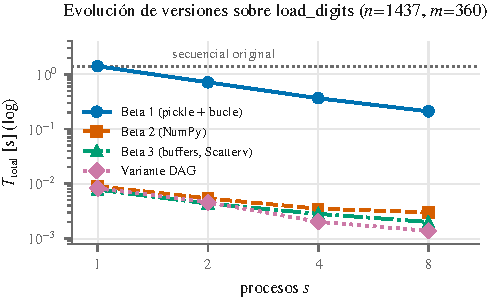
\includegraphics[width=0.62\textwidth]{f1_versiones.pdf}
\caption{Tiempo total por versión y número de procesos sobre \texttt{load\_digits}.}
\label{fig:versiones}
\end{figure}

En la Beta~1 el cómputo por consulta es muy costoso, la granularidad $G=\Tcomp/\Tcomm$ es alta y la
eficiencia con $s=8$ llega a $0.83$. La Beta~2 reduce el trabajo efectivo en dos órdenes de
magnitud al sustituir $\mte\ntr$ llamadas Python por productos matriciales; con ello
\texttt{load\_digits} se resuelve en milisegundos, la granularidad cae y la latencia de las
colectivas pasa a dominar. Esta es la justificación cuantitativa para escalar $N$ con datos
sintéticos. La Beta~3 elimina la serialización \emph{pickle} y reduce el tiempo un 33\,\% adicional
con $s=8$.

\subsection{Tiempos de ejecución, cómputo y comunicación}
\begin{figure}[H]
\centering
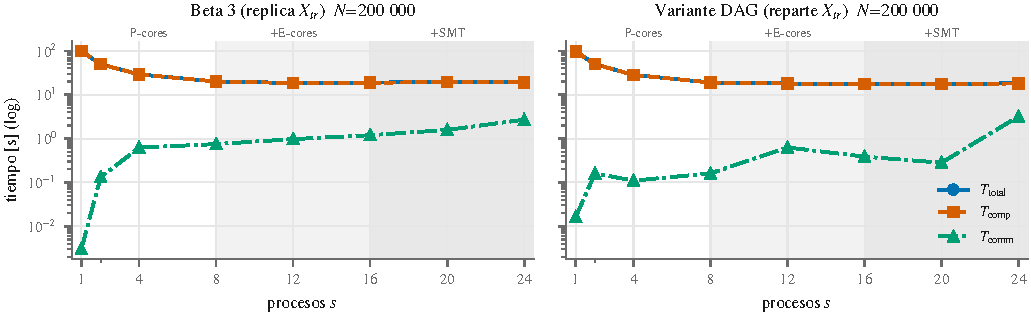
\includegraphics[width=\textwidth]{f2_tiempos.pdf}
\caption{$\Ttot$, $\Tcomp$ y $\Tcomm$ frente a $s$ con $N=200\,000$ ($\ntr=160\,000$,
$\mte=40\,000$). Las bandas sombreadas indican las regiones de hardware: hasta 8 procesos caben en
P-cores físicos; de 8 a 16 se incorporan E-cores; por encima de 16 se usan hilos SMT.}
\label{fig:tiempos}
\end{figure}

\begin{table}[H]
\centering
\caption{Escalabilidad fuerte de la Beta~3 con $N=200\,000$ (medianas).}
\label{tab:fuerte}
\begin{tabular}{rrrrrrr}
\toprule
$s$ & $\Ttot$ [s] & $\Tcomp$ [s] & $\Tcomm$ [s] & $S(s)$ & $E(s)$ & GFLOP/s\\
\midrule
1 & 98.46 & 98.46 & 0.003 & 1.00 & 1.00 & 12.5\\
2 & 49.53 & 49.51 & 0.131 & 1.99 & 0.99 & 24.8\\
4 & 29.09 & 29.06 & 0.623 & 3.39 & 0.85 & 42.3\\
8 & 19.97 & 19.93 & 0.749 & 4.93 & 0.62 & 61.7\\
12 & 18.60 & 18.54 & 0.972 & 5.29 & 0.44 & 66.3\\
16 & 18.90 & 18.80 & 1.195 & 5.21 & 0.33 & 65.4\\
20 & 19.50 & 19.39 & 1.574 & 5.05 & 0.25 & 63.4\\
24 & 19.26 & 19.11 & 2.705 & 5.11 & 0.21 & 64.3\\
\bottomrule
\end{tabular}
\end{table}

El cómputo representa más del 99\,\% de $\Ttot$ en todo el rango, lo que confirma la granularidad
gruesa obtenida en la aglomeración. Sin embargo, $\Tcomp$ deja de disminuir a partir de $s=8$: cada
proceso realiza $W/s$ operaciones pero tarda lo mismo, por lo que el límite no está en el
algoritmo sino en la plataforma. El crecimiento de $\Tcomm$ para $s\ge16$ corresponde
principalmente a espera en \texttt{Gatherv} por desbalance de carga (Sec.~\ref{sec:hw}).

\subsection{Normalización del modelo teórico y cantidad óptima de procesos}
\label{sec:norm}
\paragraph{Modelo.} A partir de la Ec.~\eqref{eq:tp}, el tiempo paralelo se expresa como la suma de
un término de cómputo y uno de comunicación, cada uno multiplicado por una constante de
normalización que convierte operaciones y palabras en segundos de esta máquina:
\begin{equation}
  T_p(s)=k_1\,\frac{W}{s}+k_2\,\Tcomm(s),\qquad W=3\,\mte\,\ntr\,d .\label{eq:norm}
\end{equation}
Para $\Tcomm(s)$ se comparan los dos modelos de comunicación vistos en clase, ``Comunicación
lineal'' y ``Comunicación en árbol (binario)''~\cite{fiestasU2}, aplicados a la difusión, que es la
colectiva dominante:
\begin{align}
  \text{árbol binario:}\quad & \Tcomm(s)=\log_2 s\,(\alpha+M\beta),\label{eq:arbol}\\
  \text{lineal:}\quad & \Tcomm(s)=(s-1)\,(\alpha+M\beta),\label{eq:lineal}
\end{align}
con $M=\ntr(d+1)+\mte d+\mte$ palabras (\texttt{Bcast} de $\Xtr,\ytr$, \texttt{Scatterv} de
$\Xte$ y \texttt{Gatherv} de $\hat{y}$).

\paragraph{Procedimiento de normalización.}
\begin{enumerate}
  \item $\alpha$ y $\beta$ se miden independientemente con colectivas sin cómputo
        (Sec.~\ref{sec:comm}), sin usar los tiempos del KNN.
  \item Para cada $N$, se calculan los regresores teóricos $x_1(s)=W/s$ y $x_2(s)=\Tcomm(s)$.
  \item $k_1$ [s/FLOP] y $k_2$ [adimensional] se obtienen por mínimos cuadrados no negativos sobre
        el $\Ttot$ medido, minimizando el error relativo
        $\sum_s\big[(k_1x_1+k_2x_2-T_{\text{med}})/T_{\text{med}}\big]^2$, pues los tiempos abarcan
        dos órdenes de magnitud.
  \item $1/k_1$ se interpreta como el rendimiento efectivo por proceso y $k_2$ como el factor por
        el que el costo real de compartir datos supera al de las colectivas aisladas.
\end{enumerate}

\paragraph{Proceso óptimo analítico.} Derivando la Ec.~\eqref{eq:norm} e igualando a cero, con
$c=\alpha+M\beta$:
\begin{align}
  \text{árbol:}\quad & -\frac{k_1W}{s^2}+\frac{k_2\,c}{s\ln 2}=0
     \;\Longrightarrow\; s^*=\frac{k_1\,W\ln 2}{k_2\,c},\label{eq:sstar-arbol}\\
  \text{lineal:}\quad & -\frac{k_1W}{s^2}+k_2\,c=0
     \;\Longrightarrow\; s^*=\sqrt{\frac{k_1\,W}{k_2\,c}} .\label{eq:sstar-lineal}
\end{align}

\begin{figure}[H]
\centering
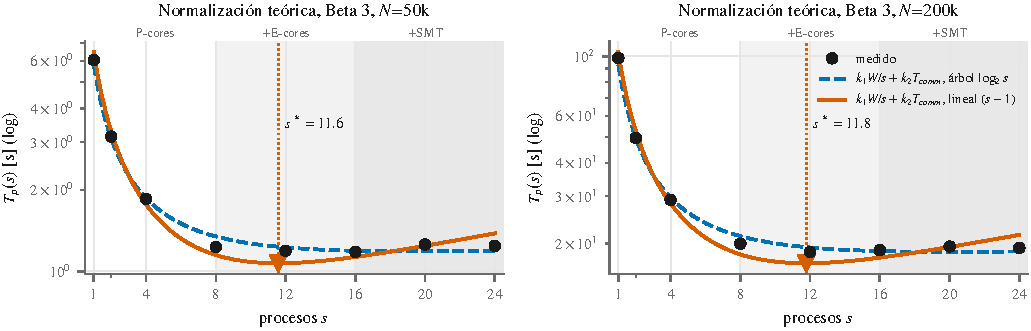
\includegraphics[width=\textwidth]{f6_modelo.pdf}
\caption{Curvas teóricas normalizadas (Ec.~\ref{eq:norm}) frente a los datos experimentales de la
Beta~3. El triángulo marca $s^*$ del modelo lineal (Ec.~\ref{eq:sstar-lineal}).}
\label{fig:modelo}
\end{figure}

\begin{table}[H]
\centering
\caption{Constantes de normalización y proceso óptimo (Beta~3).}
\label{tab:norm}
\begin{tabular}{lrrrrr}
\toprule
Modelo de $\Tcomm$ & $N$ & $k_1$ [s/FLOP] & $k_2$ & Error rel.\ medio & $s^*$\\
\midrule
\multirow{3}{*}{Árbol, Ec.~\eqref{eq:sstar-arbol}}
 & 50k  & $7.54\times10^{-11}$ & 35.6  & 3.6\,\% & 19.4\\
 & 100k & $7.41\times10^{-11}$ & 71.8  & 4.0\,\% & 18.9\\
 & 200k & $7.56\times10^{-11}$ & 139.0 & 3.4\,\% & 19.9\\
\midrule
\multirow{3}{*}{Lineal, Ec.~\eqref{eq:sstar-lineal}}
 & 50k  & $8.43\times10^{-11}$ & 31.5  & 6.2\,\% & \textbf{11.6}\\
 & 100k & $8.30\times10^{-11}$ & 63.9  & 5.7\,\% & \textbf{11.4}\\
 & 200k & $8.45\times10^{-11}$ & 122.0 & 6.4\,\% & \textbf{11.8}\\
\midrule
\multicolumn{5}{l}{Mínimo experimental $\arg\min_s\Ttot$ ($N=100$k y $200$k)} & \textbf{12}\\
\bottomrule
\end{tabular}
\end{table}

\paragraph{Discusión.}
\begin{itemize}
  \item $k_1\approx 8\times10^{-11}$\,s/FLOP equivale a $\sim$12\,GFLOP/s por proceso, el
        rendimiento medido de un P-core aislado (Sec.~\ref{sec:hw}); es estable entre tamaños.
  \item $k_2\gg 1$ y crece proporcionalmente a $N$. Si sólo se pagaran las colectivas, se esperaría
        $k_2\approx1$. El exceso indica que el costo dominante de compartir datos no está en los
        mensajes MPI, sino en la \textbf{competencia de todos los procesos por el mismo bus de
        memoria} durante el cómputo: cada proceso recorre $\Xtr$ completo (80\,MB con $N=200$k,
        más que los 30\,MB de caché L3), de modo que el tráfico de memoria es proporcional a $N$.
        Es el cuello de botella de von Neumann~\cite{backus1978,fiestasU1}: la velocidad está
        limitada por el canal procesador--memoria y no por las unidades aritméticas.
  \item Con el modelo lineal, como $W\propto N^2$ y $k_2\,c\propto N\cdot N$, el cociente de la
        Ec.~\eqref{eq:sstar-lineal} es casi independiente de $N$: $s^*\approx 11.6$ para los tres
        tamaños, en excelente acuerdo con el mínimo experimental ($s=12$). El modelo en árbol
        ajusta igual de bien los puntos medidos pero, por crecer sólo como $\log s$, no reproduce
        el aumento de $T_p$ más allá del mínimo y sitúa el óptimo en $s^*\approx 19$--$20$, en la
        zona de hilos SMT, donde los datos no muestran mejora.
  \item \textbf{Cantidad óptima estimada de procesos: $s^*\approx 12$} (8 P-cores + 4 E-cores).
        Entre $s=12$ y $s=24$ el tiempo medido varía menos de un 5\,\%, por lo que en la
        práctica conviene usar $s=12$ y no los 24 hilos disponibles: se obtiene el mismo
        resultado con la mitad de los recursos.
\end{itemize}

\subsection{Speedup y Ley de Amdahl (escalabilidad fuerte)}
\begin{figure}[H]
\centering
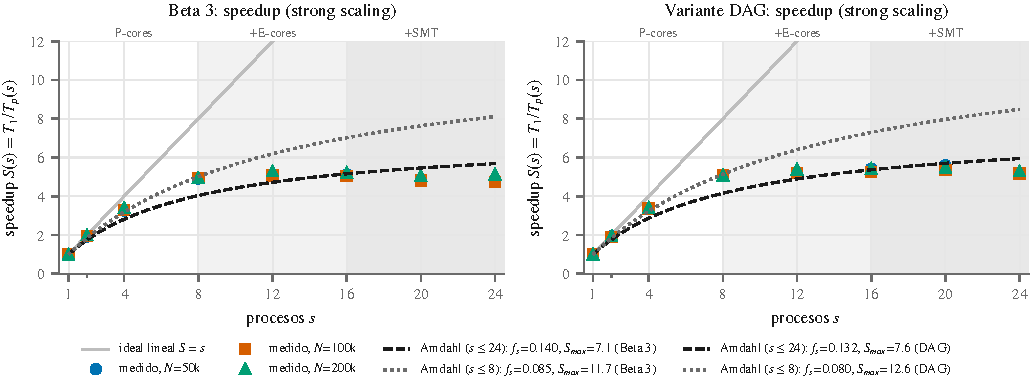
\includegraphics[width=\textwidth]{f3_speedup.pdf}
\caption{Speedup experimental $S(s)=T_1/T_p(s)$ para tres tamaños, frente al ideal lineal y a la
Ley de Amdahl ajustada en todo el rango y sólo en la región de P-cores ($s\le8$).}
\label{fig:speedup}
\end{figure}

La Ley de Amdahl~\cite{amdahl1967,fiestasU21} modela el speedup con tamaño fijo:
\begin{equation}
  S(s)=\frac{1}{f_s+\dfrac{f_p}{s}},\qquad f_s+f_p=1,\qquad
  S_{\max}=\lim_{s\to\infty}S(s)=\frac{1}{f_s}.\label{eq:amdahl}
\end{equation}
Como $T_s$ se usa la Beta~3 con $s=1$ (speedup relativo): ejecutar el secuencial original con
$N=200\,000$ tomaría $\sim$5\,h, unas $12\,400$ veces el caso de \texttt{load\_digits}. El speedup
absoluto respecto del secuencial original se reporta en la Tabla~\ref{tab:versiones}.

\begin{table}[H]
\centering
\caption{Fracción serial ajustada por la Ley de Amdahl ($N=200\,000$).}
\label{tab:amdahl}
\begin{tabular}{lcccc}
\toprule
Versión & Rango de ajuste & $f_s$ & $S_{\max}=1/f_s$ & $S$ máximo medido\\
\midrule
Beta 3 & $1\le s\le 24$ & 0.140 & 7.1 & 5.29 ($s=12$)\\
Beta 3 & $1\le s\le 8$  & 0.085 & 11.7 & 4.93 ($s=8$)\\
DAG    & $1\le s\le 24$ & 0.132 & 7.6 & 5.47 ($s=20$)\\
DAG    & $1\le s\le 8$  & 0.080 & 12.6 & 5.09 ($s=8$)\\
\bottomrule
\end{tabular}
\end{table}

Los tres tamaños de problema producen la misma curva de speedup, que se estanca en $5.1$--$5.5$.
La fracción ajustada $f_s\approx0.14$ \textbf{no corresponde a código serial}: la parte
secuencial real (\texttt{Barrier}, colectivas y cálculo de la exactitud) es menor al 1\,\% de
$T_1$. Es una \emph{fracción serial efectiva} originada por la contención del bus DDR5: los
procesos se turnan para acceder a memoria y ese acceso se comporta como una sección secuencial.
Por ello Amdahl no reproduce la forma exacta de los datos ($R^2=0.90$) y la fracción crece al
incorporar E-cores e hilos SMT ($f_s=0.085$ en $s\le8$ frente a $0.140$ en todo el rango). Que
$S(s)$ no mejore al aumentar $N$ confirma que el límite no es la comunicación MPI, cuyo peso
relativo disminuiría con $N$ según la Ec.~\eqref{eq:tp}.

\subsection{Eficiencia}
\begin{figure}[H]
\centering
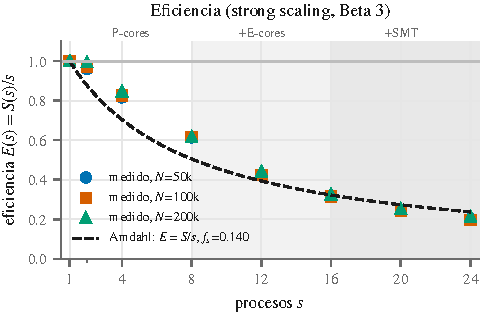
\includegraphics[width=0.62\textwidth]{f4_eficiencia.pdf}
\caption{Eficiencia $E(s)=S(s)/s$ de la Beta~3 y predicción de la Ley de Amdahl.}
\label{fig:eficiencia}
\end{figure}

De acuerdo con el análisis del informe parcial, con $\ntr$ fijo $E(s)\to0$: el algoritmo
\emph{no es fuertemente escalable} en esta plataforma. A partir de $s=12$ cada proceso adicional
aporta menos del 2\,\% de rendimiento.

\subsection{Rendimiento en FLOP/s}
\begin{figure}[H]
\centering
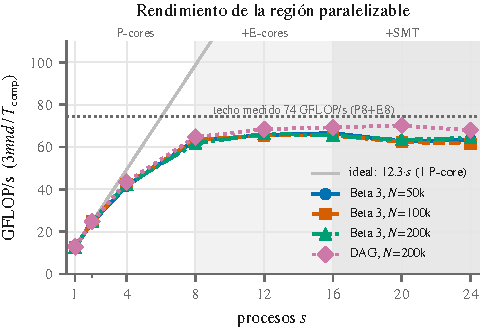
\includegraphics[width=0.62\textwidth]{f5_gflops.pdf}
\caption{GFLOP/s de la región paralelizable (Ec.~\ref{eq:flops}) frente a $s$, con el ideal
lineal de un P-core y el techo medido con afinidad explícita.}
\label{fig:gflops}
\end{figure}

El rendimiento crece casi linealmente hasta $s=8$ y se estabiliza en $63$--$66$\,GFLOP/s (Beta~3)
y $68$--$70$\,GFLOP/s (DAG), el 90\,\% del techo medido con carga equilibrada ($74.3$\,GFLOP/s).
La curva no depende de $N$: el rendimiento está determinado por los núcleos activos y su acceso
compartido a memoria, no por el tamaño del problema.

\subsection{Escalabilidad débil y Ley de Gustafson}
\begin{figure}[H]
\centering
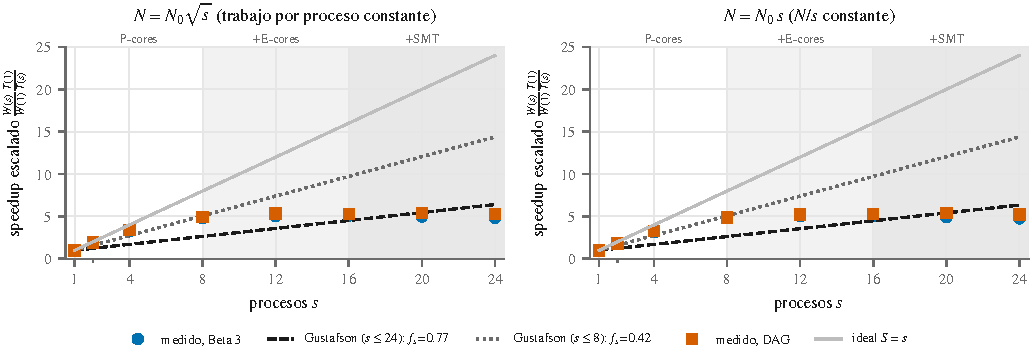
\includegraphics[width=\textwidth]{f7_debil.pdf}
\caption{Speedup escalado frente a la Ley de Gustafson. Izquierda: trabajo por proceso constante.
Derecha: $N/s$ constante.}
\label{fig:debil}
\end{figure}

La Ley de Gustafson~\cite{gustafson1988,fiestasU21} modela el speedup cuando el problema crece con
$s$:
\begin{equation}
  S(s)=f_s+s\,f_p=s-f_s\,(s-1).\label{eq:gustafson}
\end{equation}
Como el trabajo de KNN es $W=3\mte\ntr d\propto N^2$, mantener $N/s$ constante (como sugiere el
enunciado) \emph{no} mantiene constante el trabajo por proceso: $W/s\propto N_0^2\,s$ crece con
$s$. La condición de Gustafson exige $W(s)/s=W(1)$, es decir,
\begin{equation}
  N=N_0\sqrt{s}.\label{eq:nsqrt}
\end{equation}
Se midieron ambas variantes y el speedup escalado se calcula como
$S(s)=\frac{W(s)}{W(1)}\frac{T(1)}{T(s)}$, que normaliza el trabajo distinto de cada punto.

\begin{table}[H]
\centering
\caption{Escalabilidad débil de la Beta~3 con $N=N_0\sqrt{s}$ ($N_0=50\,000$).}
\label{tab:debil}
\begin{tabular}{rrrrr}
\toprule
$s$ & $N$ & $\Ttot$ [s] & Speedup escalado & $E_{\text{débil}}$\\
\midrule
1 & 50\,000 & 5.92 & 1.0 & 1.00\\
2 & 70\,711 & 6.25 & 1.9 & 0.95\\
4 & 100\,000 & 7.29 & 3.2 & 0.81\\
8 & 141\,421 & 9.84 & 4.8 & 0.60\\
12 & 173\,205 & 14.12 & 5.0 & 0.42\\
16 & 200\,000 & 18.60 & 5.1 & 0.32\\
20 & 223\,607 & 23.76 & 5.0 & 0.25\\
24 & 244\,949 & 29.36 & 4.8 & 0.20\\
\bottomrule
\end{tabular}
\end{table}

Con trabajo por proceso constante el tiempo debería mantenerse; sin embargo, se multiplica por
cinco entre $s=1$ y $s=24$. El ajuste de la Ec.~\eqref{eq:gustafson} da $f_s=0.42$ en $s\le8$ y
$0.77$ en todo el rango. Ambas variantes producen la misma curva normalizada porque miden el mismo
fenómeno: la saturación del rendimiento agregado en $\sim$65\,GFLOP/s. A diferencia de un clúster,
aumentar el problema no añade canales de memoria, de modo que la Ley de Gustafson tampoco se
cumple en esta plataforma.

Respecto de la condición de escalabilidad débil del informe parcial (Ec.~18), la comunicación
MPI sí permite crecer: con $N=N_0\sqrt{s}$ el \texttt{Bcast} de $\Xtr$ es menor al 1\,\% de
$\Ttot$ incluso con $s=24$; el resto de $\Tcomm$ es espera por desbalance de carga. El factor
limitante es el hardware compartido, no el algoritmo.

\subsection{Modelo de comunicación: árbol binario frente a lineal}
\label{sec:comm}
\begin{figure}[H]
\centering
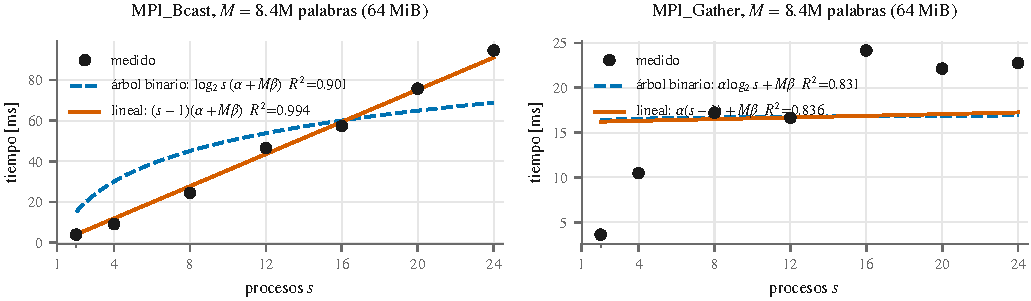
\includegraphics[width=\textwidth]{f9_comunicacion.pdf}
\caption{Tiempo de \texttt{Bcast} y \texttt{Gather} de un mensaje de 64\,MiB sin cómputo, frente a
los modelos en árbol binario y lineal ajustados con todos los tamaños de mensaje (1\,KiB--64\,MiB).}
\label{fig:comm}
\end{figure}

\begin{table}[H]
\centering
\caption{Parámetros de comunicación medidos (ajuste sobre 9 tamaños y 7 valores de $s$).}
\label{tab:comm}
\begin{tabular}{llccc}
\toprule
Colectiva & Modelo & $\alpha$ [s] & $\beta$ [s/palabra] & $R^2$\\
\midrule
\multirow{2}{*}{\texttt{Bcast}} & árbol, $\log_2 s(\alpha+M\beta)$ & $\approx0$ & $1.79\times10^{-9}$ & 0.901\\
 & lineal, $(s-1)(\alpha+M\beta)$ & $\approx0$ & $4.72\times10^{-10}$ & \textbf{0.994}\\
\midrule
\multirow{2}{*}{\texttt{Scatter}} & árbol, $\alpha\log_2 s+M\beta$ & $8.2\times10^{-5}$ & $1.23\times10^{-9}$ & 0.867\\
 & lineal, $\alpha(s-1)+M\beta$ & $2.9\times10^{-5}$ & $1.22\times10^{-9}$ & 0.873\\
\midrule
\multirow{2}{*}{\texttt{Gather}} & árbol, $\alpha\log_2 s+M\beta$ & $1.4\times10^{-4}$ & $1.94\times10^{-9}$ & 0.831\\
 & lineal, $\alpha(s-1)+M\beta$ & $4.7\times10^{-5}$ & $1.93\times10^{-9}$ & 0.836\\
\bottomrule
\end{tabular}
\end{table}

En clase se presentaron dos modelos~\cite{fiestasU2}: la \emph{comunicación lineal}, en la que la
raíz envía el mensaje a cada proceso por turno, con $T_{\text{bcast}}=O\big(p(\alpha+m\beta)\big)$ y
$T_{\text{scatter/gather}}=O(\alpha p+\beta m)$; y la \emph{comunicación en árbol (binario)}, con
$T_{\text{bcast}}=O\big(\log p\,(\alpha+m\beta)\big)$ y $T_{\text{scatter/gather}}=O(\alpha\log p+\beta m)$.
El modelo en árbol es menor porque en cada etapa se duplica el número de procesos que retransmiten
el mensaje por enlaces independientes~\cite{grama2003,thakur2005}. En la
máquina de este proyecto, el \texttt{Bcast} de 64\,MiB tarda $3.9$\,ms con $s=2$ y $94.5$\,ms con
$s=24$: crece $\sim$24 veces, lo que corresponde a $O(s)$ y no a $O(\log s)$ ($\log_2 24/\log_2 2
\approx 4.6$). El modelo lineal explica el 99.4\,\% de la varianza frente al 90.1\,\% del árbol.

La razón es que en memoria compartida no existen enlaces independientes: Intel MPI implementa las
colectivas intranodo como copias a través de memoria compartida~\cite{intelmpi}, y las $s-1$ copias
del mensaje compiten por el mismo canal DDR5. El costo total es entonces $(s-1)M\beta$, con un
ancho de banda efectivo por copia de $8/\beta\approx17$\,GB/s. Es otra manifestación del cuello de
botella de von Neumann~\cite{backus1978}: lo que en un clúster se paralelizaría en la red, aquí se
serializa en el bus de memoria. En \texttt{Scatter} y \texttt{Gather} el término dominante es
$M\beta$, común a ambos modelos ($T=O(\alpha p+\beta m)$ frente a $O(\alpha\log p+\beta m)$), por lo
que los dos ajustan de forma similar ($R^2\approx0.83$--$0.87$); su variabilidad restante proviene
de la sincronización con el proceso más lento.

En el KNN, el \texttt{Bcast} de $\Xtr$ con $N=200$k (83\,MB) cuesta $0.15$\,s con $s=24$, sólo el
0.8\,\% de $\Ttot$; la comunicación explícita no es el cuello de botella, pero el mismo mecanismo
---competencia por el bus de memoria--- es el que, durante el cómputo, satura el rendimiento
(Sec.~\ref{sec:norm}).

\subsection{Justificación de hardware: núcleos P, núcleos E y SMT}
\label{sec:hw}
\begin{figure}[H]
\centering
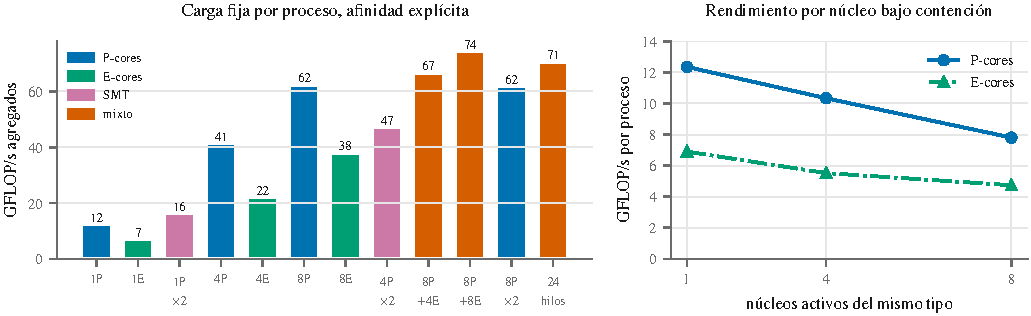
\includegraphics[width=\textwidth]{f8_pinning.pdf}
\caption{Rendimiento con la misma carga por proceso ($1024$ consultas $\times$ $160\,000$ puntos)
y afinidad explícita a P-cores, E-cores o hilos SMT. Izquierda: GFLOP/s agregados.
Derecha: GFLOP/s por proceso al aumentar los núcleos activos del mismo tipo.}
\label{fig:pinning}
\end{figure}

El material del curso advierte sobre este fenómeno en la diapositiva ``procesos vs.\ hilos''
de la Unidad~4~\cite[p.~22]{fiestasU4}:
\begin{quote}\itshape
``No se recomienda usar todos los hilos de un CPU por proceso porque más hilos por proceso no
significa más rendimiento. Pasado cierto punto, cada hilo extra aporta poco o incluso resta.
Debido a: Ancho de banda de memoria (\ldots{} tiene muchísimos más hilos que canales para
alimentarlos), NUMA, SMT (Simultaneous Multithreading) no equivale a núcleos reales, Sobrecarga de
OpenMP/MPI y Desbalance de carga. El óptimo suele estar en un punto intermedio\ldots''
\end{quote}
Para verificar experimentalmente estos factores se fijó cada proceso a una CPU lógica concreta con
la misma carga de trabajo. Los resultados confirman tres de ellos (el i7-14650HX tiene un único
nodo de memoria, por lo que NUMA no aplica, y la sobrecarga de MPI ya se midió como menor al 1\,\%
en la Sec.~\ref{sec:comm}):

\begin{enumerate}
  \item \textbf{Saturación del ancho de banda de memoria.} Un P-core aislado rinde
        $12.3$\,GFLOP/s, pero baja a $10.3$ con 4 P-cores activos y a $7.8$ con 8; los E-cores
        pasan de $6.9$ a $4.7$. El rendimiento de cada núcleo disminuye cuando otros usan la
        memoria a la vez, aunque cada uno tenga su propio núcleo físico.
  \item \textbf{SMT no equivale a núcleos reales.} Dos procesos en los dos hilos de un mismo
        P-core suman $16.1$\,GFLOP/s, apenas un 30\,\% más que uno solo. Ocho procesos en 4 P-cores
        con SMT rinden $47.0$, frente a $62.2$ en 8 P-cores físicos. Pasar de 16 a 24 procesos
        (agregando los hilos SMT) no mejora el rendimiento ($74.3\to70.6$).
  \item \textbf{Desbalance de cargas (P-cores frente a E-cores).} Un E-core rinde la mitad que un
        P-core ($6.9$ frente a $12.3$\,GFLOP/s). Con reparto por bloques iguales, en la
        configuración 8P+8E los procesos en E-cores rinden $3.2$\,GFLOP/s y los de P-cores
        $6.0$: el tiempo total lo fija el más lento y los rápidos esperan en \texttt{Gatherv}.
        Esto explica el crecimiento de $\Tcomm$ medido para $s\ge12$ (Tabla~\ref{tab:fuerte}),
        que es principalmente espera y no transferencia.
\end{enumerate}

El óptimo medido, $s^*=12$, es exactamente el ``punto intermedio'' que anticipa la diapositiva: ni
los 8 P-cores ni los 24 hilos. Las tres regiones de la Fig.~\ref{fig:tiempos} quedan así explicadas: hasta $s=8$ escalan los
P-cores, limitados por el ancho de banda compartido; de $8$ a $16$ los E-cores aportan poco y
desbalancean la carga; por encima de $16$ los hilos SMT comparten unidades de ejecución y no
añaden rendimiento.

\subsection{Comparación de descomposiciones: Beta 3 frente a variante DAG}
\begin{table}[H]
\centering
\caption{Beta~3 (replica $\Xtr$) frente a variante DAG (reparte $\Xtr$), $N=200\,000$.}
\label{tab:dag}
\begin{tabular}{rrrrrr}
\toprule
 & \multicolumn{2}{c}{$\Ttot$ [s]} & \multicolumn{2}{c}{$\Tcomm$ [s]} & \\
\cmidrule(lr){2-3}\cmidrule(lr){4-5}
$s$ & Beta 3 & DAG & Beta 3 & DAG & Fusión DAG [s]\\
\midrule
1  & 98.46 & 96.52 & 0.003 & 0.016 & 0.006\\
8  & 19.97 & 19.03 & 0.749 & 0.161 & 0.018\\
12 & 18.60 & 18.01 & 0.972 & 0.626 & 0.025\\
16 & 18.90 & 17.82 & 1.195 & 0.387 & 0.043\\
24 & 19.26 & 18.23 & 2.705 & 3.187 & 0.056\\
\bottomrule
\end{tabular}
\end{table}

La variante DAG es entre un 2 y un 6\,\% más rápida y alcanza más GFLOP/s ($70$ frente a $66$).
Dos factores lo explican: (i) evita el \texttt{Bcast} de $\Xtr$, que bajo el modelo lineal cuesta
$(s-1)\ntr d\beta$; y (ii) cada proceso recorre sólo $\ntr/s$ puntos de entrenamiento, por lo que su
bloque de datos es $s$ veces menor y reduce el tráfico hacia memoria, el recurso que limita la
escalabilidad. Su fusión serial crece linealmente con $s$, como predice la Ec.~\eqref{eq:tdag},
pero con $k=3$ es despreciable ($0.056$\,s con $s=24$). Ambas versiones producen predicciones
idénticas.

\subsection{Límites de escalabilidad y mejoras propuestas}
\begin{itemize}
  \item \textbf{Límite principal:} el ancho de banda de memoria compartido. Aumentar los procesos
        por encima de $s^*\approx12$ no reduce el tiempo en esta máquina.
  \item \textbf{Balance dinámico o ponderado:} asignar a cada proceso un número de consultas
        proporcional a su rendimiento (P-core $\approx2\times$ E-core) en \texttt{Scatterv},
        reduciendo la espera en \texttt{Gatherv}.
  \item \textbf{Afinidad explícita:} con $s\le8$, fijar los procesos a P-cores físicos evita que el
        sistema operativo los asigne a hilos SMT o E-cores.
  \item \textbf{Bloqueo por caché:} recorrer $\Xtr$ en bloques que quepan en la caché L2 y
        reutilizarlos para varias consultas aumenta la intensidad aritmética y alivia el bus.
  \item \textbf{Memoria distribuida:} en un clúster, cada nodo aporta su propio canal de memoria y
        la variante DAG eliminaría la réplica de $\Xtr$; allí el modelo en árbol sería el adecuado
        y la escalabilidad débil mejoraría según la Ley de Gustafson.
\end{itemize}

% ============================================================================
\section{Conclusiones}
% ============================================================================
\begin{enumerate}
  \item Se paralelizó KNN con MPI siguiendo PCAM y un diseño PRAM CREW, expresado con el formalismo
        \texttt{forall}~\ldots~\texttt{pardo} en los Algoritmos~\ref{alg:knn-pram}--\ref{alg:knn-dag}.
        Las tres versiones beta y la variante DAG producen las mismas predicciones que el código
        secuencial y que scikit-learn.
  \item El desarrollo en versiones mostró que la vectorización (Beta~2) reduce el tiempo
        $\sim$156 veces y la comunicación con buffers (Beta~3) un 33\,\% adicional; el speedup
        absoluto frente al código original llega a $\sim$700 (Beta~3) y $\sim$1000 (DAG) con 8 procesos.
  \item La normalización $T_p(s)=k_1W/s+k_2\Tcomm(s)$ con el modelo de comunicación lineal reproduce
        los datos con un 6\,\% de error y predice analíticamente $s^*\approx11.6$, en acuerdo con el
        mínimo experimental $s=12$, que es la cantidad óptima de procesos estimada.
  \item El speedup se satura en $\sim$5.3 ($f_s\approx0.14$ según Amdahl), con eficiencia $0.21$
        para $s=24$; la escalabilidad débil tampoco se sostiene (Gustafson, $E=0.20$ con $s=24$). La
        causa, demostrada experimentalmente, no es la comunicación MPI sino el hardware compartido:
        saturación del ancho de banda de memoria, SMT que no equivale a núcleos reales y desbalance
        entre P-cores y E-cores.
  \item En memoria compartida las colectivas siguen el modelo lineal $O(s)$ ($R^2=0.994$) y no el
        de árbol binario: las copias compiten por el bus DDR5, una manifestación directa del cuello
        de botella de von Neumann.
\end{enumerate}

% ============================================================================
\section{Bibliografía y uso de fuentes externas}
% ============================================================================
Esta sección detalla qué fuente se empleó, con qué propósito y su impacto en el trabajo.

\subsection{Material del curso}
El material de clase de Fiestas~\cite{fiestasU1,fiestasU2,fiestasU21,fiestasU22,fiestasU3,fiestasU4} define
el marco teórico y la notación de todo el informe:
\begin{itemize}
  \item Unidad~1~\cite{fiestasU1}: DAG, taxonomía de Flynn, metodología de Foster (Sec.~2.2) y el
        cuello de botella de von Neumann usado para interpretar $k_2$ y el modelo lineal.
  \item Unidad~2.1~\cite{fiestasU21}: speedup, eficiencia, FLOPs, Ley de Amdahl (escalabilidad
        fuerte, Ec.~\ref{eq:amdahl}) y Ley de Gustafson (escalabilidad débil, Ec.~\ref{eq:gustafson}).
  \item Unidad~2~\cite{fiestasU2}: diapositivas ``Comunicación lineal'' y ``Comunicación en árbol
        (binario)'' (págs.~7--8), base de las Ecs.~\ref{eq:arbol}--\ref{eq:lineal}, de la
        normalización de la Sec.~\ref{sec:norm} y del contraste experimental de la
        Sec.~\ref{sec:comm}.
  \item Unidad~2.2--2.3~\cite{fiestasU22}: PRAM CREW, formalismo \texttt{pardo} y teorema de Brent.
  \item Unidad~3~\cite{fiestasU3}: colectivas MPI (\texttt{Bcast}, \texttt{Scatter(v)},
        \texttt{Gather(v)}) usadas en los Algoritmos~\ref{alg:knn-mpi}--\ref{alg:knn-dag}.
  \item Unidad~4~\cite{fiestasU4}: diapositiva ``procesos vs.\ hilos'' (pág.~22), citada
        textualmente en la Sec.~\ref{sec:hw}; sus factores (ancho de banda de memoria, SMT,
        desbalance de carga) se verificaron experimentalmente con el estudio de afinidad.
  \item Enunciado del proyecto~\cite{fiestasProyecto}: código secuencial, DAG de referencia y
        preguntas de análisis.
\end{itemize}

\subsection{Literatura científica y documentación técnica}
\begin{itemize}
  \item Fix y Hodges~\cite{fix1951}, Cover y Hart~\cite{cover1967}: fundamento de KNN y de su
        naturaleza no paramétrica, que concentra el cómputo en la consulta.
  \item JáJá~\cite{jaja1992} y Brent~\cite{brent1974}: PRAM CREW, sintaxis \texttt{pardo} y cota
        del tiempo paralelo (Ec.~\ref{eq:brent}).
  \item Grama et al.~\cite{grama2003} y Thakur, Rabenseifner y Gropp~\cite{thakur2005}: costo de
        las colectivas en árbol, contrastado con nuestras mediciones (Sec.~\ref{sec:comm}).
  \item Valiant~\cite{valiant1990} y Culler et al.~\cite{culler1993}: motivación de modelos con
        costo explícito de comunicación (BSP, LogP).
  \item Foster~\cite{foster1995}, Flynn~\cite{flynn1972}, Amdahl~\cite{amdahl1967} y
        Gustafson~\cite{gustafson1988}: metodología PCAM, clasificación MIMD/SPMD y leyes de
        escalabilidad.
  \item Backus~\cite{backus1978}: formulación del cuello de botella de von Neumann.
  \item Pacheco~\cite{pacheco2011} y Quinn~\cite{quinn2003}: referencia de programación MPI.
  \item Aparicío, Blanquer y Hernández~\cite{aparicio2007}: validan la estrategia de replicar
        $\Xtr$ y repartir las consultas; Patwary et al.~\cite{patwary2016} y Xiao y
        Biros~\cite{xiao2016}: cuellos de botella de KNN distribuido a gran escala.
  \item Documentación técnica: mpi4py~\cite{mpi4pydoc,dalcin2021} (semántica de \texttt{Bcast},
        \texttt{Scatterv}, \texttt{Gatherv} con buffers), Intel MPI~\cite{intelmpi} (colectivas
        intranodo), Intel~\cite{intelark} (arquitectura del i7-14650HX), Microsoft~\cite{mscpuset}
        (topología P/E), scikit-learn~\cite{pedregosa2011} (validación), NumPy~\cite{harris2020},
        SciPy~\cite{virtanen2020} (ajustes por mínimos cuadrados) y Matplotlib~\cite{hunter2007}
        (figuras).
\end{itemize}

\subsection{Uso de herramientas de asistencia y modelos de lenguaje}
En cumplimiento de las pautas del curso, se declara el uso del modelo de lenguaje Claude~\cite{claude},
a través del entorno Claude Code, como herramienta de apoyo.

\printbibliography[heading=bibintoc,title={Referencias}]

\end{document}
